\documentclass{llncs}


\usepackage{subfigure}
\usepackage{graphicx}


\title{A Graphical Notation for \\ Physical Database Modelling}
\author{Antonia Pillay\inst{1} \and Nigel Stanger\inst{2}}
\institute{???? Malaysia \and Department of Information Science, University of Otago, Dunedin, New Zealand \email{nstanger@infoscience.otago.ac.nz}}


\begin{document}


\maketitle


\begin{abstract}
In this paper we describe a graphical notation for physical database
modelling. This notation provides database administrators (DBAs) with a
means to model the physical structure of new and existing databases,
thus enabling them to make more proactive and informed tuning decisions,
compared to existing database monitoring tools.
\end{abstract}


\section{Introduction}

As with most information systems, the design and implementation of a
database goes through several phases, including conceptual, logical and
physical modelling \cite{BeDa-P-2003}. These three phases are of
particular interest, as they embody the progression from higher to lower
levels of abstraction \cite{Tsic-D-1978}. Conceptual models are
typically highly abstract, using techniques such as entity-relationship
modelling. Logical models represent the database structure in a form
that is closer to the physical representation, yet still sufficiently
abstract to isolate applications from the physical representation
\cite{Codd-EF-1970}, and are expressed using formalisms such as the
relational model. A logical model for a database can be derived by
transforming the corresponding conceptual model.

Physical models represent the database structure in terms of the
physical storage implementation of a specific database management system
(DBMS) such as Oracle or DB2. A physical model for a database can be
derived by transforming the corresponding logical model
\cite{Bato-DS-1985,Conn-TM-2002}. Because of their low abstraction
level, physical level database models have tended to not be expressed
using graphical notations, unlike models at higher levels of
abstraction.

Physical level modelling, however, is equally as important as, if not
\emph{more} important than the higher levels, because it is the physical
level that determines the performance of a database \cite{BeDa-P-2003}.
It is somewhat surprising that there have been relatively few attempts
to devise a graphical physical modelling notation, because such a
notation can provide several advantages
\cite{Conn-TM-2002,BeDa-P-1992-PDD,Will-J-1992}:
\begin{itemize}

	\item it can reduce complexity and thus improve understandability
	\cite{Tuft-ER-1997};

	\item it can provide a more complete and integrated display of
	performance tuning techniques in a database;

	\item database developers can be more confident about the design
	decisions that they make for the performance of the database;

	\item database performance problems are more easily visualised
	using a graphical notation; and

	\item a specific methodology is developed and used, thus enabling
	developers to resolve physical performance issues more
	systematically.

\end{itemize}

These benefits are embodied in modern database performance monitoring
tools, which provide higher-level visualisations of a database's
internals in order to easily identify and highlight performance
problems. Such tools, however, are primarily \emph{monitoring} tools
rather than \emph{design} tools. They may therefore unintentionally
encourage DBAs into a \emph{reactive} mode of continually ``tweaking''
the database to resolve performance issues, rather than a
\emph{proactive} mode of anticipating and designing for expected usage.
It may also be difficult for a DBA using such tools to gain a clear and
comprehensive overview of all the tuning techniques that are in use
within a particular database \cite{Core-MJ-1997-OracleDW}.

In this paper we propose a graphical notation for physical database
modelling. In Sect.~\ref{sec-techniques}, we provide a brief overview of
commonly used physical tuning techniques. We then discuss in
Sect.~\ref{sec-previous} two earlier approaches upon which our work is
partially based. Sect.~\ref{sec-notation} introduces our proposed
notation, and Sect.~\ref{sec-future} discusses possible future work. The
paper concludes in Sect.~\ref{sec-conclusion}.


\section{Physical Tuning Techniques}
\label{sec-techniques}

Database management is generally an I/O bound task, so the main
performance bottleneck in most databases will be the speed of offline
storage such as disk drives. Retrieving data from a hard disk is
theoretically about six orders of magnitude slower than retrieving data
from RAM\footnote{On the order of milliseconds (\(10^{-3}\)) for disk
versus nanoseconds (\(10^{-9}\)) for RAM.}. The aim of any physical
tuning strategy must therefore be to minimise the impact of slow
storage, either by directly reducing the number of physical disk
accesses required, or by parallelising access to disk in order to reduce
contention.

These considerations have led to the development of five general
physical tuning techniques, which are implemented to various degrees by
most modern mainstream DBMS products:

\begin{description}

	\item[Indexes] reduce the number of physical disk accesses required
	to retrieve a specific record, most typically by building a B+-tree
	\cite{Knut-DE-1997-Art} based on some key value. Without any
	indexes, a DBMS often has little choice but to perform a sequential
	scan in order to locate a specific record.

% A common database operation is to request a specific data record
% identified by a some key value. When such a request occurs, the DBMS
% must locate this record on disk (assuming that it is not already cached
% elsewhere). If we assume that the records are randomly ordered with
% respect to the chosen key value, then the DBMS has no option but to
% perform a sequential scan of all the records, which will require on
% average\(n/2b\) disk accesses, where \(n\) is the number of records and
% \(b\) is the number of records per database block (the worst case is
% \((n - 1)(b)\)). Sorting the records on the key value will obviously
% help for searches based on that key value, but will not help for
% searches based on a different key value.
% 
% One solution is to build a separate index structure that associates key
% values with their corresponding physical record. Because indexes are
% stored separately, we can provide multiple indexes on different key
% values for the same set of records. In addition, by choosing an
% appropriate data structure for the index, we can improve the efficiency
% of searching and thus reduce the number of physical disk accesses
% required \cite{Roti-S-1996}. Most modern DBMSs use some variant of the
% \emph{B+-tree} structure \cite{Knut-DE-1997-Art}. This structure has
% average and worst case performance of (formula) and (formula),
% respectively.
% 
% Indexes are a ``pure'' disk access minimisation technique, that is, they
% reduce the number of physical disk accesses required, but do not provide
% any form of paralellism. B-tree indexes perform well for a wide range of
% typical database queries (ref), but can suffer in high update
% environments due to the need to also update the index.

	\item[Hashing] is a method of quickly locating specific records by
	passing a key value to a \emph{hash function}. This function returns
	the physical location of a hash bucket, which contains a pointer to
	the associated physical record (check). Hashing schemes typically
	require only a single disk access to retrieve a specific record.

% Hashing is another pure disk access minimisation technique that performs
% well for exact key queries on very large tables. Rather than build a
% separate index structure, a key value is passed to a \emph{hash
% function}. This function returns the physical location of a hash bucket,
% which contains a pointer to the associated physical record (check).
% Hashing schemes typically require only a single disk access to retrieve
% a specific record, but perform poorly for queries that require the
% retrieval of multiple records.

	\item[Clustering] minimises disk access by ensuring that related
	records (such as an order header and its associated order lines) are
	physically adjacent on disk. This usually means that related records
	will be stored in the same database block, and can thus be retrieved
	with a single disk access.

% Clustering is a disk access minimisation technique that can be applied
% when two different record types are logically related, and thus commonly
% retrieved together; for example, an order header and its order lines.
% Without any further optimisation, such an operation could at worst
% require one disk access for the order header and one disk access for
% each of its order lines.
% 
% To improve this situation, we \emph{cluster} the two record types, so
% that related physical records are physically adjacent to each other
% \cite{Chan-N-2003-clustering}. This usually means that all the records
% will be stored in the same database block, and can thus all be retrieved
% with a single disk access. Clustering can, however, be expensive to
% maintain in a high update environment.

	\item[Partitioning] provides parallel access paths to data by
	physically splitting a table into disjoint parts and placing them on
	separate disks. This is particularly advantageous when multiple
	users wish to access different subsets of a set of records, because
	it provides a separate physical access path to each of the
	partitions.
% 	Partitioning can also reduce the number of disk accesses
% 	required, because there are fewer records to scan in each partition
% 	than if the table were not partitioned.

% In a typical untuned database, all data will be stored on the same disk.
% If the database is heavily accessed, then contention for the single I/O
% channel to this disk becomes a major bottleneck. Partitioning reduces
% this contention by splitting the database into disjoint partitions, each
% of which is assigned to a different disk. This approach is particularly
% advantageous in situations where multiple users wish to access different
% subsets of a set of records, because it provides a disjoint physical
% access paths to each of the partitions. This reduces I/O channel
% contention and thus improves performance. Partitioning is thus primarily
% an access parallelism technique.
% 
% Partitioning can also provide some disk access minimisation benefits,
% because the amount of data to be searched in each partition is smaller
% than if the database were not partitioned.

	\item[Replication] provides parallel access paths to data by making
	multiple copies of the same records and placing them on separate
	disks. This is particularly advantageous when multiple users need to
	access the same sets of records, but is more complex to manage due
	to the need to keep replicas synchronised.

% Replication is an access parallelism technique in which multiple copies
% of the same records are placed on different disks, thus providing
% multiple physical access paths to the same data.

\end{description}

These techniques are normally applied to different parts of a database
to achieve different effects. In order to choose an appropriate physical
tuning technique, the DBA must consider various factors that may benefit
only some users of the database, or may improve the performance of the
database as a whole. While most of the techniques can be combined to
varying degrees, simply applying all techniques is usually not optimal,
because each technique excells under different conditions. That is, what
are optimal conditions for one technique may be the exact opposite for
another, so the DBA needs to be able to model all the available
information in order to develop an appropriate physical design.



\section{Prior Physical Modelling Techniques}
\label{sec-previous}

To achieve an effective physical design requires a large amount of
information, particularly with regard to the predicted or actual volume
and usage of data within the database \cite{BeDa-P-2003}. Incorporating
this information into a graphical model can provide a more concise and
clearer overview of the physical aspects of a database system. In this
section we briefly discuss two previous efforts at modelling such
information in a graphical manner.


\subsection{Agile Modeling (Ambler)}

Ambler proposed a physical modelling notation based on the Unified
Modeling Language (UML), as part of a larger effort to produce a
``traditional'' style data modelling profile for the UML
\cite{Ambl-SW-2003-ADT,Ambl-SW-2004-ObjPrimer3}. Ambler and others have
argued the need for such a profile for some time
\cite{Ambl-SW-1998-BOA,Naib-EJ-2001-UMLDD}.

Ambler's notation focuses on the physical modelling of relational
databases. The notation uses class boxes without stereotypes to
represent physical tables, while indexes are represented by class boxes
with the stereotype \verb|<<index>>|, as illustrated in
Fig.~\ref{fig-Ambler}. There appear to be no stereotypes for other
physical tuning techniques such as partitioning, although these could be
easily incorporated.

\begin{figure}
	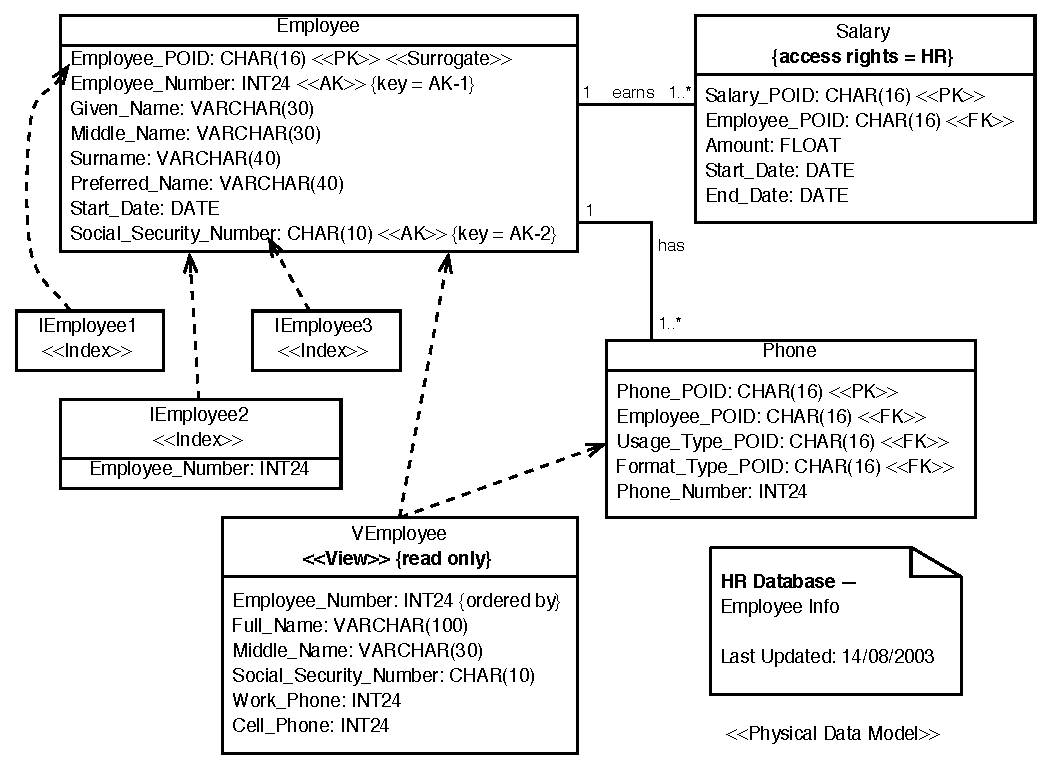
\includegraphics[width=\columnwidth,keepaspectratio]{Ambler}
	\caption{Ambler's physical modelling notation (adapted from \cite{Ambl-SW-2003-ADT})}
	\label{fig-Ambler}
\end{figure}

Ambler's approach suffers from two serious disadvantages. First, the
notation is very limited in the types of symbol used. All physical
level constructs are represented by class boxes, which in a complex
diagram could make distinguishing them difficult. This limitation
probably arises from the constraints on developing a new notation within
the existing UML framework.

Second, his approach appears to consistently confuse the logical and
physical levels of abstraction: the same notations are used to represent
not only physical but also logical and conceptual elements
\cite{Ambl-SW-2003-ADT}. This confusion is illustrated by the inclusion
of a view (a non-physical construct) in Fig.~\ref{fig-Ambler}.

In summary, while Ambler's notation does graphically model the physical
level of a database, the similarity of the graphical symbols and the
evident confusion between the physical and logical levels diminish its
usefulness.

% . He states that since Unified
% Modelling Language (UML) does not cover data (i.e., ER) modelling yet,
% he presents the solution in this paper. Ambler has argued for some time
% for the presence of data modelling in UML \cite{Ambl-SW-1998-BOA}, and
% has suggested various ways that it should be done. It is enlightening to
% know that Ambler is not alone in his quest for adopting an industry
% standard in data modelling. Other methodologies like
% \cite{Naib-EJ-2001-UMLDD} have recognized the need as well. This model
% type is built on the practice of UML 2.0 of separating core methodology.
% Ambler admits that the methodology that he has presented is not perfect
% and it focuses on the physical modelling of a relational database. In
% this model he also tries to stress style issues that according to him
% are not appropriate for a proper UML profile \cite{Ambl-SW-2003-ADT}.

% This model suggests that a class box without a stereotype in a physical
% database design is a table. It also represents views that have
% dependencies on the table structures. Tables, entities and views are all
% modelled using class boxes. The class boxes that appear on the logical
% and conceptual model are entities so the stereotype is optional.
% Similarly, it is assumed that any class box without a stereotype on a
% physical data model is a table. Ambler's methodology seems to be limited
% in terms of annotations. All representations whether tables or indices
% are modelled using class boxes. This representation can sometimes be
% confusing and exact identification of tables and indices in the system
% has to be known by the database designer. In this model, relationships
% are modelled using associations that are derived from the logical data
% model. He further discusses his methodology for modelling attributes and
% columns, keys, constraints and triggers, stored procedures and sections.
% Ambler states that requirements for something should be identified
% before it is built. He states the requirements of each model, e.g.,
% requirements that are needed to model entities and tables, requirements
% that are needed to model relationships, etc.
% 
% An example of Ambler's notation is shown in Fig.~\ref{fig-Ambler}.

% Even though a lot of detail is covered in his suggestion, Ambler's
% methodology somehow seems relatively weak. It is much too general in
% annotations and has no specific description. The methodology seems to
% consistently confuse the logical and physical design. For example: both
% are modelled using class boxes but are later explained as representing
% different objects. However, this model will definitely be useful as a
% stepping-stone to work towards an official UML data modelling profile.


\subsection{Physical Design Using an Entity Model (Beynon-Davies)}

Beynon-Davies proposed a method for analysing and modelling the physical
usage patterns of a database \cite{BeDa-P-1992-PDD}. In his method,
various aspects of the physical performance of a database are measured,
such as the size and expected growth rates of tables (volume analysis),
the volatility of tables, and the frequency of transactions (usage
analysis). The data obtained from these analyses are then used to
annotate a logical level entity-relationship diagram (ERD) of the
database, producing what is known as a \emph{composite usage map} (see
Fig.~\ref{fig-Beynon-Davies} on page~\ref{fig-Beynon-Davies} for an
example).

Beynon-Davies' method provides a very good mechanism for representing
the usage statistics of database in a coherent manner, but is somewhat
complex to execute without some form of automation. Our experience with
teaching this method at undergraduate level shows that even with a
relatively small database, the designer can quickly become overwhelmed
by the sheer volume of usage data involved.

In addition, Beynon-Davies' method does not produce any conclusions as
to which physical tuning methods should be implemented---rather it
provides much of the information required to enable these decisions to
be made. Beynon-Davies' method is thus more a notation for summarising
the physical usage patterns of a database, rather than a notation for
physical modelling per se.

% The closest model that demonstrates the link between conceptual, logical
% and physical design work is by Beynon-Davies \cite{BeDa-P-1992-PDD}. He
% suggests a method that can be used for the physical design process. The
% paper defines physical modelling as ``the transformation of the logical
% model into a definition of the physical model suitable for a specific
% software/hardware configuration'' \cite{BeDa-P-1992-PDD}.
% 
% According to Beynon-Davies one of the first steps that must be taken to
% move from logical to physical database design is to establish estimates
% of the average and maximum number of instances per entity (volume
% analysis). Volatility analysis is represented in the same way. Similar
% to volume analysis, volatility analysis cannot be used as a measure if a
% table is continually growing. It is most effective if the size of the
% table is static. Figure 9 summarizes Beynon-Davies's final modelling
% method; he does not model all the individual annotations but generalizes
% the entity relationship diagrams into a general model.
% 
% It is understandable that the reason behind this generalization is to
% minimize complexity and since individual annotations are developed in
% the beginning, references can be made to them if needed. This might be
% effective for small systems that have a limited number of tables.
% However, for medium to large-scale projects, Beynon-Davies suggests that
% a systematic analysis of volatility and usage should be done. This
% analysis would constitute a map of the database application that would
% be maintained by the DBA. This meets the objective of providing an
% overview of all the performance tuning techniques and data in place.


\section{A New Physical Notation}
\label{sec-notation}

Both of the notations discussed in the previous sections are limited in
their ability to graphically model the physical level of a database.
Ambler's notation lacks clarity and is thus potentially confusing, while
Beynon-Davies' notation only summarises the physical usage patterns of a
database rather than providing an actual physical level database model.
We have therefore adopted aspects from both approaches to devise a
graphical notation that enables database designers to graphically model
the common physical database tuning techniques discussed in
Sect.~\ref{sec-techniques}.

The notations that we have adopted for this notation are shown in
Fig.~\ref{fig-notation}. Some of these are adapted from other notations,
while some we have created ourselves. The symbols have been chosen to be
intuitive and simple to draw, so as to produce diagrams that are as
clear and uncluttered as possible. Physical models may be developed
using this notation either with or without a prior Beynon-Davies style
analysis.

\begin{figure}
	\centering
	\subfigure[Table]{\label{fig-notation-table}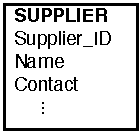
\includegraphics[scale=0.9]{notation-table}}
	\hfill
	\subfigure[Indexes]{\label{fig-notation-index}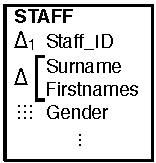
\includegraphics[scale=0.9]{notation-index}}
	\hfill
	\subfigure[Hashing]{\label{fig-notation-hash}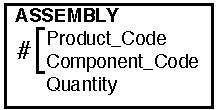
\includegraphics[scale=0.9]{notation-hash}}	\\
	\subfigure[Clustering]{\label{fig-notation-cluster}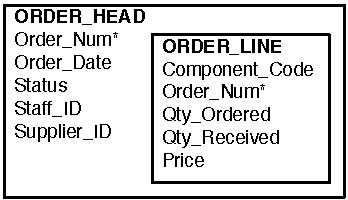
\includegraphics[scale=0.9]{notation-cluster}}
	\hfill
	\subfigure[Partitoning]{\label{fig-notation-partition}\includegraphics[scale=0.9]{notation-partition}}
	\hfill
	\subfigure[Replication]{\label{fig-notation-replica}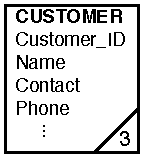
\includegraphics[scale=0.9]{notation-replica}}
	\caption{Proposed notations for physical tuning techniques}
	\label{fig-notation}
\end{figure}

A physical table is represented by a simple box, as shown in
Fig.~\ref{fig-notation-table}. This is similar to most logical and
conceptual level ERD notations. The fields of the physical table may be
included, with or without physical data types, as appropriate.

Indexes are represented by a small tree-like symbol within a table, as
shown in Fig.~\ref{fig-notation-index}. The index key is listed next to
this symbol. Composite keys are indicated by a grouping symbol. Hashing
is represented in a similar way, but uses an ``H'' symbol instead of a
tree symbol (see Fig.~\ref{fig-notation-hash}).

Clustering is represented by nesting one table inside another, as shown
in Fig.~\ref{fig-notation-cluster} (adapted from
\cite{BeDa-P-1992-PDD}). The cluster key is indicated by an asterisk (*)
attached to the appropriate field(s). Tables may be nested to as many
levels as required in order to represent more complex clustering
schemes. This notation is intuitive, and clearly indicates the field(s)
on which the records are clustered.

Partitioning is represented by splitting a table into either vertical or
horizontal partitions according to the style of partitioning, as shown
in Fig.~\ref{fig-notation-partition} (adapted from
\cite{Silb-A-2002-4E}). Once again, the notation is intuitive, and
allows the partition definitions to be easily indicated.

Replication is indicated by placing a diagonal bar across the
bottom-right corner of the table to be replicated, along with the total
number of replicas, as shown in Fig.~\ref{fig-notation-replica}. This is
adapted from a similar notation used in data flow diagrams
\cite{Gane-C-1979}. This notation could also be used to indicate
replication of individual table partitions, for DBMSs that permit this
combination.

% The graphical notations use in this model is not complex and cluttered.
% This is to enable a database designer to simplify the physical design in
% a notation that will be easy to understand but comprehensive. Some of
% the graphical notations use in this model was adapted from other models
% and a few were modified by the author to suit the model.
% 
% The table below illustrates some of the graphical representations that
% were available to choose from.

Consider the entity-relationship diagram shown in Fig.~\ref{fig-ERD},
which uses Martin notation \cite{Mart-J-1990-IE2} to depict a database
for a consumer electronics manufacturer. A corresponding Beynon-Davies'
composite usage map based on the fourteen most significant transactions
is shown in Fig.~\ref{fig-Beynon-Davies}. The arrows represent physical
access paths, while the number attached to each access path indicates
the number of disk accesses per hour along that path. The diagram
clearly highlights some potential performance problem areas in the
database, for example:
\begin{itemize}

	\item There are many disk accesses on the access paths between the
	Sale\_head/Sale\_line and the Order\_head/Order\_line tables. Since
	these are tables that will normally be accessed together, both could
	perhaps be candidates for clustering (depending on the mix of update
	versus read operations).

	\item The appear to be multiple transactions acessing the Staff
	table. This could imply a need for partitioning.
	
	\item There is an extremely high access rate on the Customer table.
	Further examination, however, reveals that this rate only occurs for
	a short period once per month, and that the transaction in question
	only requires read access. Replication of the Customer table could
	therefore be a suitable solution.
	
\end{itemize}

\begin{figure}
	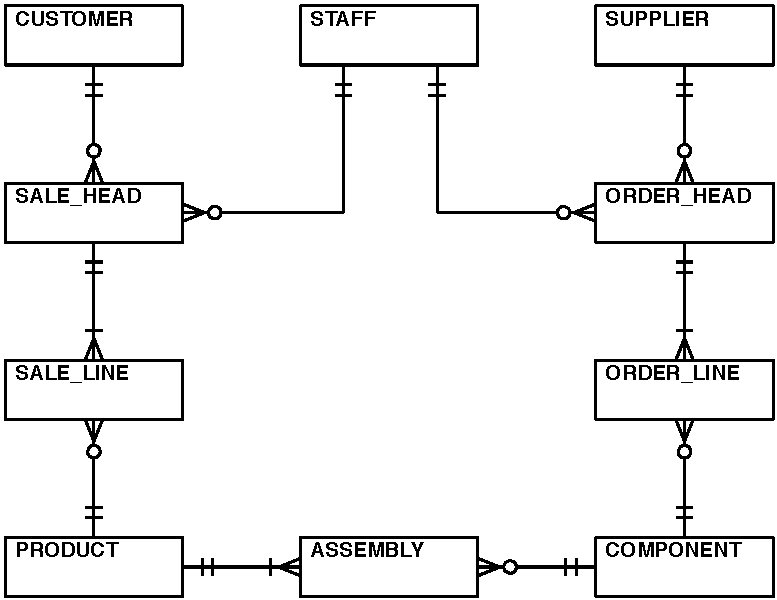
\includegraphics[width=\columnwidth,keepaspectratio]{ERD}
	\caption{ERD of the example database}
	\label{fig-ERD}
\end{figure}

\begin{figure}
	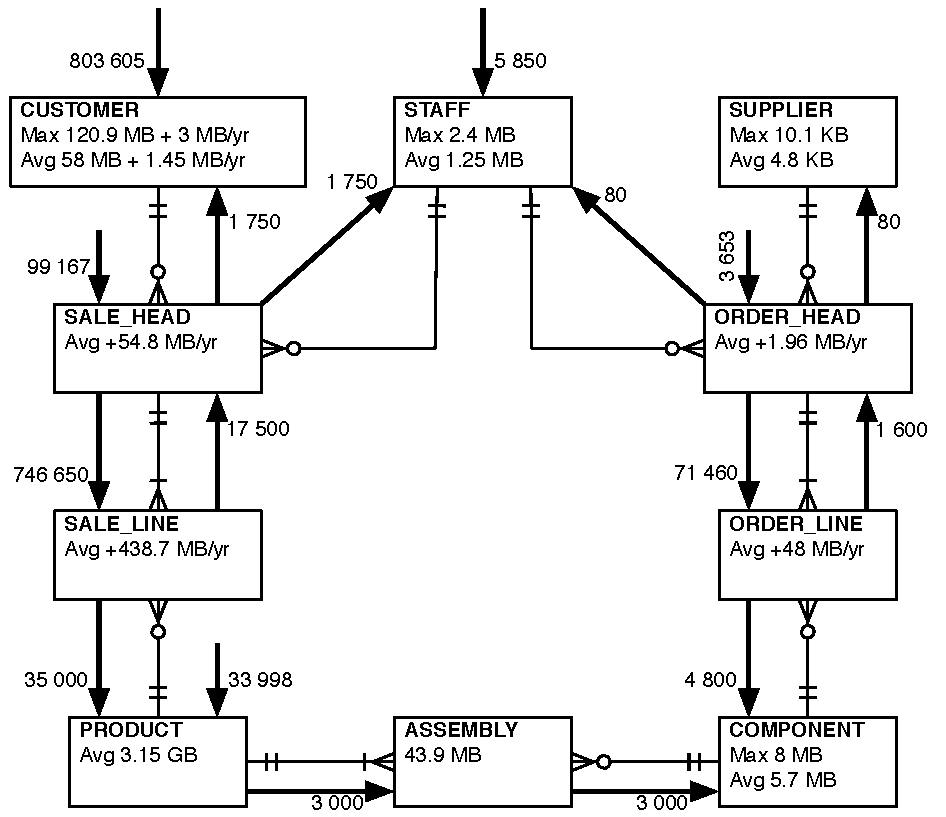
\includegraphics[width=\columnwidth,keepaspectratio]{Beynon-Davies}
	\caption{Beynon-Davies composite usage map for the example database}
	\label{fig-Beynon-Davies}
\end{figure}

The suggestions above can be represented as a physical model using our
proposed modelling notation, as shown in Fig.~\ref{fig-physical-model}
(some details have been omitted to save space). Note that we have placed
indexes on all primary keys as a matter of course.

\begin{figure}
% 	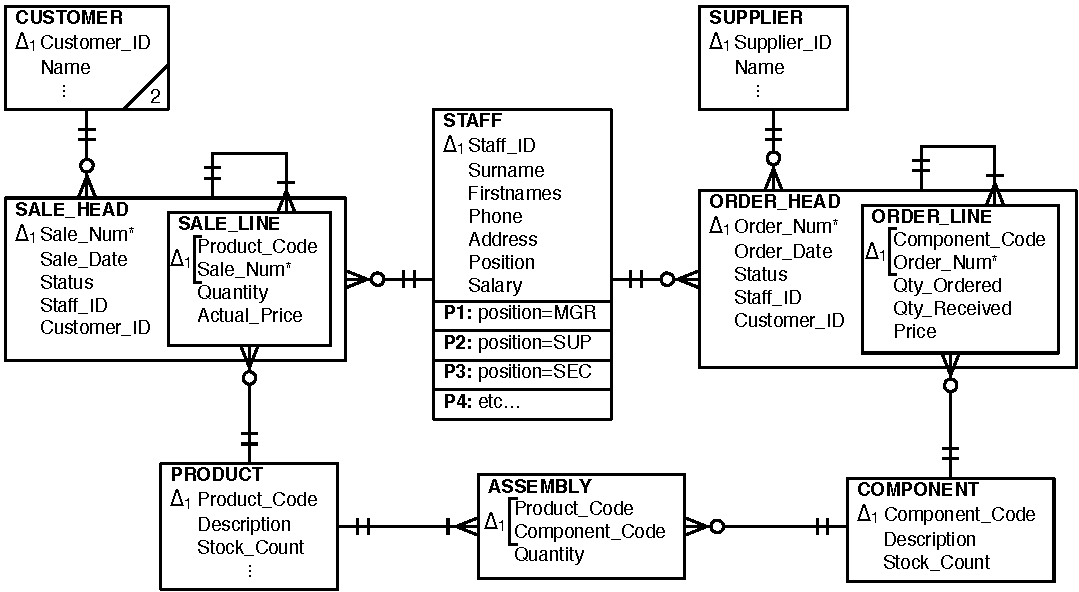
\includegraphics[angle=90,scale=0.9]{Physical-Model}
	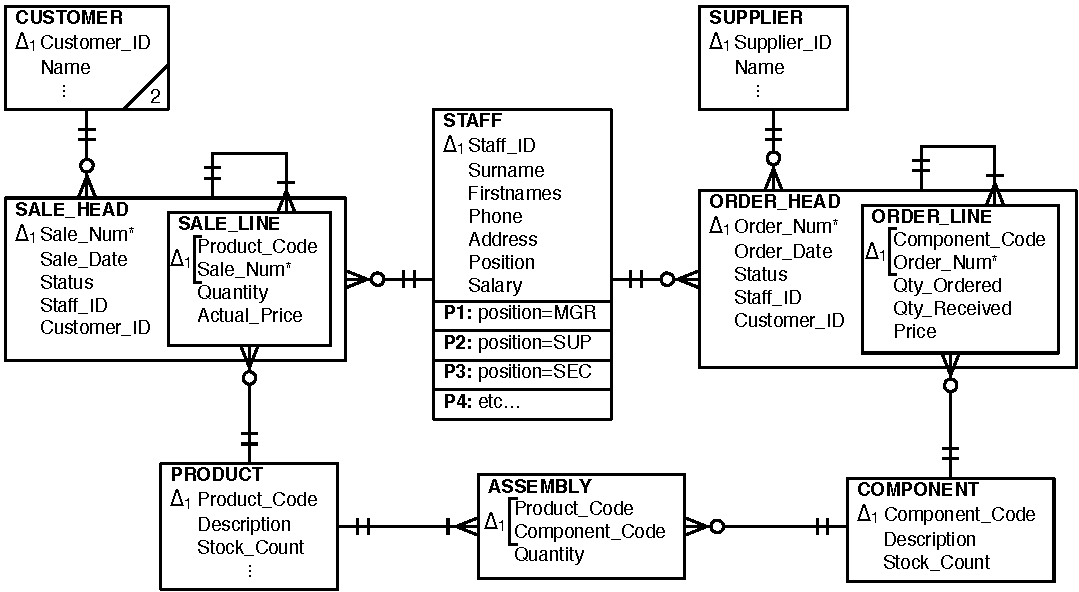
\includegraphics[width=\columnwidth,keepaspectratio]{Physical-Model}
	\caption{Physical database model for the example database}
	\label{fig-physical-model}
\end{figure}


\section{Future Research}
\label{sec-future}

- symbols for different types of index (reverse-key, index-organised
tables, R-trees, bitmap indexes).

- physical placement information, i.e., what devices partitions go on, etc.

- evaluation of the notation with undergraduate students \& comparison
with Beynon-Davies (preliminary results by time of publication).


\section{Conclusion}
\label{sec-conclusion}


\bibliographystyle{splncs}

\bibliography{ER2005}


\end{document}
